\documentclass[12pt,a4paper]{article}
\usepackage[utf8]{inputenc}
%\usepackage[hidelinks]{hyperref}
\usepackage{caption}
\usepackage{hyperref}
\usepackage{xcolor}
\usepackage{cite}
\usepackage[version=4]{mhchem} % for isotope symbols
\usepackage{a4wide}
\usepackage[lmargin=2cm,rmargin=2cm,tmargin=2cm,bmargin=2cm,headheight=0in]{geometry}
\usepackage{amssymb}
\usepackage{graphicx}


\hypersetup{colorlinks, linkcolor={blue!50!black}, citecolor={blue!50!black},
	urlcolor={blue!50!black}}
	
% Caption font sizes	
\DeclareCaptionFont{CaptionFontSize}{\fontsize{12pt}{12pt}}
\captionsetup[table]{font=CaptionFontSize}
\captionsetup[figure]{font=CaptionFontSize}

\begin{document}
%\title{Nuclear isomers for energy storage and fundamental physics} - broad
%\title{Investigation of the energy storage potential of $\ce{^{113m}Cd}$ using time-correlated gamma ray-coincidence spectroscopy}% - narrower
%\title{Investigation of $\ce^{{113m}Cd}$ for energy storage and the physics of breakup in nuclear reactions} - narrowest
%\title{Investigation of $\ce{^{148,150,152}Ce}$ and $\ce{^{113m}Cd}$ using time-correlated gamma ray-coincidence spectroscopy}
\title{Searching for octupole collectivity in neutron-rich Ce isotopes and isomer depletion pathways in $\ce{^{113}Cd}$} % Working title
\author{Student: Caspian Nicholls (u1027945)}
\date{Supervisor: Dr. A. J. Mitchell, Department of Nuclear Physics, Research School of Physics and Engineering, Australian National University}
%\date{\today}

% From AJ
%Title: Probably needs to change. Something like “Search for octupole collectivity in neutron-rich Ce isotopes and isomer depletion pathways in 113Cd” ? 
%
%Context and aims: Opening paragraph to explain the situation of project change, then broader context. Set out the timeline of La decay analysis now until end of June. Reassess. Cd experiment ~ August (?) if possible. If this is set out clearly, then the rest can follow more easily. 
%

\maketitle
\section*{Context and Aims}
%General introduction to the field of nuclear physics
\medskip
Nuclear physics is first and foremost the study of nuclei, of which there are hundreds. Among the various experimental and theoretical projects being undertaken in this field, there are researchers performing experiments to try and understand the patterns of nuclear structure that exist across the chart of nuclides. One such phenomenon exhibited by isotopes with neutrons numbers N around 88 is that of strong octupole collectivity: long-range interactions between nucleons that reside in orbitals separated by three units of both orbital and total angular momentum. Predictions based on models of nuclear structure have been made for the range of nuclides that should exhibit this behaviour, but it has not been experimentally observed for each isotope in this list.

\medskip
At the same time, a dedicated research campaign is being undertaken to assess the potential of excited states of certain isotopes with relatively long half-lives (known as \textit{nuclear isomers} or metastable states) for storing large amounts of energy in a space-efficient manner over long periods of time. 

\medskip
The original plan was to perform experiments at the start of May to collect data for an exploration centred around $\ce{^{113}Cd}$. Preparations for these experiments were already well underway. However, given the restrictions on access to experimental equipment instated by the ANU in response to the global COVID-19 pandemic, these preparations have had to be halted. Hence, the first stage of this project will now comprise an investigation of yet unanalysed experimental data collected during an experiment with the aim of exploring the structure of isotopes $\ce{^{148,150,152}Ce}$. These nuclides have N $ = 90$, $92$ and $94$ respectively and are thus expected to exhibit strong octupole collectivity. 

\medskip
This stage will extend until the end of June, at which point the progress of this project will be re-assessed to determine whether experiments to study $\ce{^{113}Cd}$ are worthwhile. This second stanza of the project would comprise making new measurements to search for isomer depletion pathways within the structure of $\ce{^{113}Cd}$ and explore its energy storage potential. If possible, the experiments for this study will be performed sometime in July or August to allow time for analysis of the resulting data.

\subsection*{Octupole collectivity}

\medskip
%motivate your project and identify what problem you are solving or what you will be doing.
The correlations associated with octupole collectivity are one key factor that governs the level schemes of different nuclides. Most isotopes that exhibit this property have mass numbers A in the vicinity of either 146 or 222. Nuclei of Ce with N$\sim$88 fall into the former category, having traits linked to the presence of significant octupole correlations, rendering them as intriguing cases from which we can learn about nuclear structure.

\medskip
However, currently only some of the excitation energies and lifetimes of the low lying negative-parity states of $\ce{^{148,150,152}Ce}$ are known. Measuring values of these quantities enables determination of the quadrupole and dipole moments for these nuclides, which in turn allows their quadrupole and octupole collectivity to be assessed. By analysing gamma ray spectra recorded using an array of gamma ray detectors (known as Gammasphere) this project aims to make measurements of these quantities and thus gauge the afore-mentioned collectivities for these isotopes. 
Ideally, this will include the first measurement of octupole collectivity in $\ce{^{150}Ce}$.
For the ground state of $\ce{^{152}La}$, determination of its lifetime and placing bounds on its spin are some additional goals of this part of the project.
Doing so will enhance the existing understanding of octupole correlations displayed by the low spin excited states of these cerium nuclei.

% To do: refine/include aims for octupole collectivity bit.

\subsection*{Nuclear isomers}

\medskip
By and large, excited states of atomic nuclei release their excess energy on femtosecond time scales. Yet, there exist long-lived excited nuclear states with half-lives up to 30 orders of magnitude greater than this~\cite{shaffer_innovations_2018}. The typical energy densities of these isomers are around $10^9$~J/g, approximately five orders of magnitude higher than the limit placed on chemical means of energy storage (fuels, batteries, food) by the binding energy between particles ($\lesssim 100$~eV).

\medskip
For the goal of harnessing this dense energy source, many nuclear isomers with half-lives on the order of years (or greater) have been identified as potentially useful. The question for each such metastable, however, is are there ways by which this energy can be released? Current work in this field is centred around searching for a reaction pathway that will cause the isomer to dispense its energy by moving into a lower energy state.

\medskip
The leading suggestion for such a reaction pathway is that of isomer depletion. In this process, a sample containing some nuclear isomer is exposed to a beam of high-energy photons. If the isomer absorbs a photon that has the appropriate energy to excite the isomer to a state with a much shorter half-life, then the isomer will decay (via either a single gamma ray transition, or a cascade of multiple gamma ray emissions) to the ground state of that isotope. This process was first reported when a sample of the isomer $\ce{^{180m}Ta}$ was excited to a so-called depletion level (or intermediate state) in 1988, demonstrating that the energy of these isomers can be released on demand~\cite{collins_depopulation_1988}. The decay of the metastable state was followed by the decay of the ground state, which resulted in a total of $~780$~keV being emitted. 

\medskip
However, the energy required to initiate this depletion process was $~$1000~keV, prompting investigation of other isomers with half-lives in excess of one year, of which ten others have been identified for an ongoing research campaign~\cite{shaffer_innovations_2018}. % Mention this ongoing research campaign is being conducted by ARL here? 
With funding provided as part of this campaign, this project aims to experimentally study the isomer $\ce{^{113m}Cd}$ (with energy 263.54~keV above the ground state and a half-life of 14.1~yr) of the isotope $\ce{^{113}Cd}$, with the primary goal of identifying such an energy-releasing pathway. As part of this overarching aspiration, there are the sub-goals of gaining expertise in gamma ray spectroscopy, nuclear instrumentation and the operation of the 14UD tandem accelerator located at the ANU. In addition, I am to develop my skills in analysing multi-parameter data sets that will be generated as a result of the experimental part of this project. Finally, I aim to meaningfully interpret the results of this analysis under the framework of a range of theoretical models of nuclear structure.

% Other possible aims:
% measuring cross sections
% Investigating break up

\section*{Background}

\subsection*{Octupole collectivity}
% To do (will be strongly based on research proposal for the experiment itself given it clearly explains a lot of the background). Can just cite this as a 
% Octupole collectivity comes about from octupole-octupole (like dipole-dipole but higher order) interaction between nucleon (either proton or neutron - see details from AJ) orbitals that are separated by three units of total and orbital angular momentum.
% Protons: h_{11/2} and d_{5/2} orbitals
% neutrons: i_{13/2} and f_{7/2} orbitals
% s: l=0, p: l=1, d: l=2, f: l=3, g: l=4, h: l=5, i: l=6
% might need to explain spectroscopic notation here

%Background: Describe the caribu project, radioactive beams, nuclear shapes, octupole deformation, Ba examples. Transition into experiment work at ANU, isomer program etc 

\medskip
\subsection*{Nuclear isomers}
% Why do excited states of nuclei exist
\medskip
The nucleons contained within nuclei preferentially arrange themselves into the most stable (lowest energy) configuration, which is known as the ground state.
Nuclei are split into three categories (even-even, odd-even or odd-odd) based on the numbers of protons ($Z$) and neutrons ($N$) they possess and the parities of each.
The configuration of the nucleons within the nucleus is referred to in terms of the spin-parity (denoted $J^\pi$ where $J$ is the magnitude of the total angular momentum of the nucleus and $\pi$ represents its parity in three dimensional space). 
% Worth explaining what parity is? Would non-specialist physicists know this? Anyone who took physics of matter or QM should, but not everyone will have... I am going to take it as understood for now
Where possible, nucleons try and pair up (typically with other like nucleons, i.e. protons (neutrons) with protons (neutrons)) to form coupled states with $J^\pi = 0^+$. 
Excited states generally arise in one of three ways: either the coupling between a pair of nucleons is broken, an unpaired nucleon in a given nuclear orbital is excited into a higher lying orbital, or some combination of these two effects occurs. 
These excited states may or may not have a different spin-parity to the ground state, but they are always more energetic.
% Is this too much detail?
% Do I need to mention the differences between vibrational and rotational states? Collective motion vs single particle states? Maybe not here, but probably will be required for the full thesis as context for any level schemes that are included/discussed.

% Why do isomers exist?
\medskip
Due to these energy differences, transitions between different nuclear states are accompanied by either the absorption or emission of a photon. However, based on the principles of quantum mechanics, there are \textit{selection rules} that govern (in terms of the quantum numbers of the initial and final nuclear states) which transitions are allowed.
Some states are metastable because there are no lower energy states that they are allowed to decay into in light of these fundamental physical rules.
% at the very least, their half-life is either really long or their decays are slow enough to have never been observed...
In general, nuclear isomers exist because the decay of the isomeric state is inhibited. 
One possible reason for this inhibition is that the difference in the total angular momentum of the nuclear state before and after the transition (referred to as the multipolarity, $\Delta J$) is relatively large.
This is because transitions with large $\Delta J$ values are known to be slow in comparison to those with lower multipolarities.

\medskip
The long-lived isomer $\ce{^{113m}Cd}$ exhibits one such high multipolarity transition, shown in Figure~\ref{fig:cd113} as the only photon line between the isomer at 263.54 keV and the ground state.
The E5 notation is a shorthand way of expressing that the gamma radiation field for this transition has odd parity ($\pi = (-1)^5  = -1$) and carries (orbital) angular momentum of magnitude $5\hbar$. This is because the isomer has $J^\pi = 11/2^-$ and the ground state has $J = 1/2^+$, giving $\Delta J = 5\hbar$ and $\Delta \pi = -1$.
There are no other (known) transitions by which this isomer can decay to the ground state~\cite{j._blachot_nucl._data_sheets_111_1471_2010_data_extracted_from_the_ensdf_database_revision_of_june_2010._notitle_nodate}.
% Although there could be a possible isomer depletion pathway, but it has not been commented on I think.
% Worth explaining why its called multipolarity? It's to do with the electric (or magnetic) multipole moment of the photon transition.
% May need to add some references to Krane or other textbooks here.

\begin{figure}
	\centering
	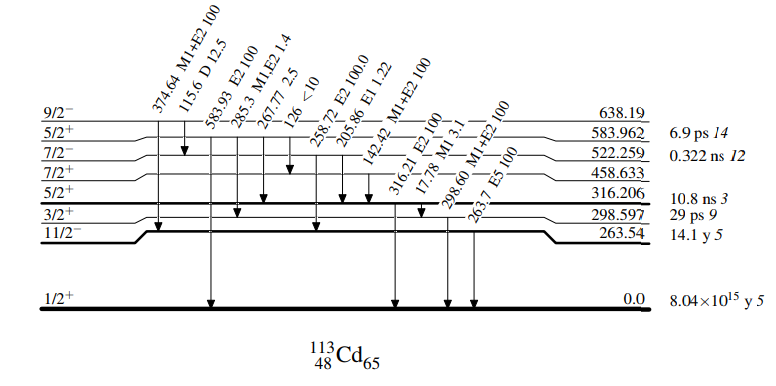
\includegraphics[width=0.9\textwidth]{113cd_partial_level_scheme_ENSDF.png}
	\caption{Partial level scheme for $\ce{^{113}Cd}$. The isomeric state has an energy of 263.54~keV~\cite{j._blachot_nucl._data_sheets_111_1471_2010_data_extracted_from_the_ensdf_database_revision_of_june_2010._notitle_nodate}.}
	\label{fig:cd113}
\end{figure}

% Previous work on isomer depletion
% Up to here.



%"Background information necessary to understand my particular project".
%\begin{itemize}
%\item Why do nuclear isomers exist? Vibrations, rotations, collective motion. Selection rules and forbidden photon transitions. From physics of matter (lecture 26 Greg), nuclear isomers exist because the decay of the isomeric state is inhibited, generally from a combination of the following factors:
%\begin{itemize}
%\item The state can only decay (by spontaneous emission) via a high multipolarity gamma-ray transition, which are known to be relatively slow (compared to lower multipolarity transitions). It could be this for 113Cd, as the spin-parity of the isomer is 11/2$^-$ whilst the ground has $J^\pi = 1/2^+$ (E5 or M6 transition since there is a change in parity).
%\item The most probable decay path is a very low energy transition - the Weisskopf estimates show that low energy transitions are strongly inhibited.
%\item The wavefunction overlap between the parent and daughter wavefunction is very small, inhibiting the decay.
%\end{itemize}
%\item Energy level scheme for cadmium 113.
%\item The process of isomer depletion. What is an intermediate state/depletion level? - covered
%\item Breakup phenomenon. Why breakup occurs (because of the cluster structures of 7Li and 9Be).
%\item What is a cross section?
%% more to come...



\section*{Project Description}

%Project description: need to think about this 

\section*{Project Plan and Feasibility}

%Project plan: need to think about this
%
%Feasibility: Do-able. 

%\vspace*{-\baselineskip}
\bibliographystyle{ieeetr}
\bibliography{references.bib}{}
% No more than 20 refs


\end{document}